 																							                               	%---Orsay---%
%%%%%%%%%%%%%%%%%%%%%%%%%%%%%%%%%%%%%%%%%%%%%%%%%%%%%%%%%%%%%%%%%%%%%%%%%%%%%%%%%%%%%%%%%%%%%%%%%%

\documentclass[a4paper,11pt]{article}

%---Packages utilisés
\usepackage[utf8]{inputenc}
\usepackage[T1]{fontenc}
\usepackage[frenchb]{babel}
\usepackage{indentfirst}
\usepackage[]{graphicx}
\usepackage{amsmath}
\usepackage{ccaption}
\usepackage{vmargin}
\usepackage{textcomp}
\usepackage{fancyhdr}
%\usepackage[avantgarde]{quotchap}
\usepackage[Lenny]{fncychap}
\usepackage{cite}

\fancypagestyle{plain}{
\fancyhead[]{}
\fancyfoot[R]{\thepage}
\renewcommand{\headrulewidth}{0pt}}

%---Nouvelles commandes
\newcommand{\cyrce}{\textsc{Cyrcé}}
\newcommand{\Root}{\textsc{Root}}
\renewcommand{\baselinestretch}{1.2}
\newcommand{\alp}{$\alpha$}
\newcommand{\Asta}{$^{211}$At}
\newcommand{\AstaIso}{$^{210}$At}

%\renewcommand{\chaptermark}[1]{%
% \markboth{\thechapter . \ #1}{}}

%---Mise en page
\setlength{\parindent}{2ex}
%\pagestyle{fancy}

%---Début du document
\begin{document}

%---Marges du document
\setmarginsrb{3.5cm}{1.5cm}{1.5cm}{2cm}{2ex}{3ex}{2ex}{5ex}
%1 est la marge gauche
%2 est la marge en haut
%3 est la marge droite 
%4 est la marge en bas
%5 fixe la hauteur de l'etête
%6 fixe la distance entre l'entte et le texte
%7 fixe la hauteur du pied de page
%8 fixe la distance entre le texte et le pied de page
%
%\chapterstyle{veelo}
%\renewcommand{\sectionmark}[1]{\markright{\thesection\ #1}}
\lhead[]{}
\fancyfoot[C]{}
\fancyfoot[R]{\thepage}

%%%%%%%%%%%%%%%%
\begin{center}
\subsection*{Analyse des données issues des irradiations à Orsay (CPO-Kinétron)}
\end{center}

\subsection*{Rappel de l'ensemble des irradiations}
\begin{center}
\begin{tabular}{ll}
Fichier&Notes\\
\hline
\hline
Double\_dosion\_kinetron\_1&Deux Dosion placés à la suite (3~mm devant)\\
Double\_dosion\_kinetron\_ate\_100\_1&Idem + atténuateur 100 branché sur le 3~mm\\
Double\_dosion\_kinetron\_ate\_100\_2&Idem mais intensité 16 à 20 fois supérieure\\
Double\_PM\_1&Uniquement 3 mm avec PM -- 50~V (grille)\\
Double\_PM\_2&80~V (grille)\\
Double\_PM\_3&90~V (grille)\\
Double\_PM\_4&100~V (grille)\\
Double\_PM\_5&150~V (grille)\\
Double\_PM\_6&150~V (grille)\\
\hline
\end{tabular}
\end{center}

Le faisceau du Kinétron est pulsé, avec une largeur fixée à 0,1~$\mu$s pour toutes les irradiations exceptée la dernière où elle était de 1~$\mu$s, et une fréquence choisie à 100~Hz.
L'énergie en sortie est fixe à 4,5~MeV.

\subsection*{Calibrer Dosion}

Les intensités étant trop élevées pour placer le PM directement dans le faisceau, nous ne pouvons calibrer Dosion de la sorte. 
Pour l'instant, nous utiliserons des valeurs obtenues théoriquement à l'énergie de sortie des électrons, à savoir : 
$$\text{Calib}=0,009574\text{ fC/part.}$$
$$\text{TEL}=1,882\text{ MeV/cm}$$
La valeur de calibrage donnée est celle pour 3~mm d'air, car comme nous le verrons, aucune mesure réalisée n'était exploitable pour le 5~mm.
Le TEL est celui dans l'eau.

\subsection*{Analyse des fichiers}

Comme dit précédemment, des problèmes de saturation des électromètres ont rendu impossible une analyse fine des mesures effectuées sur les Dosion non équipés d'atténuateur.
\`A titre d'exemple, voici les résultats obtenus, figure \ref{fig:area_sat}, pour le Dosion de 3~mm lors de la première irradiation.
Nous y distinguons des pistes -- 25 et 26 suivant X et 13 suivant Y -- dont les résultats semblent incohérents, mais en réalité c'est l'ensemble des points qu'il convient de remettre en doute tant le comportement des électromètres saturés est imprévisible.
\begin{figure}[h]
\begin{center}
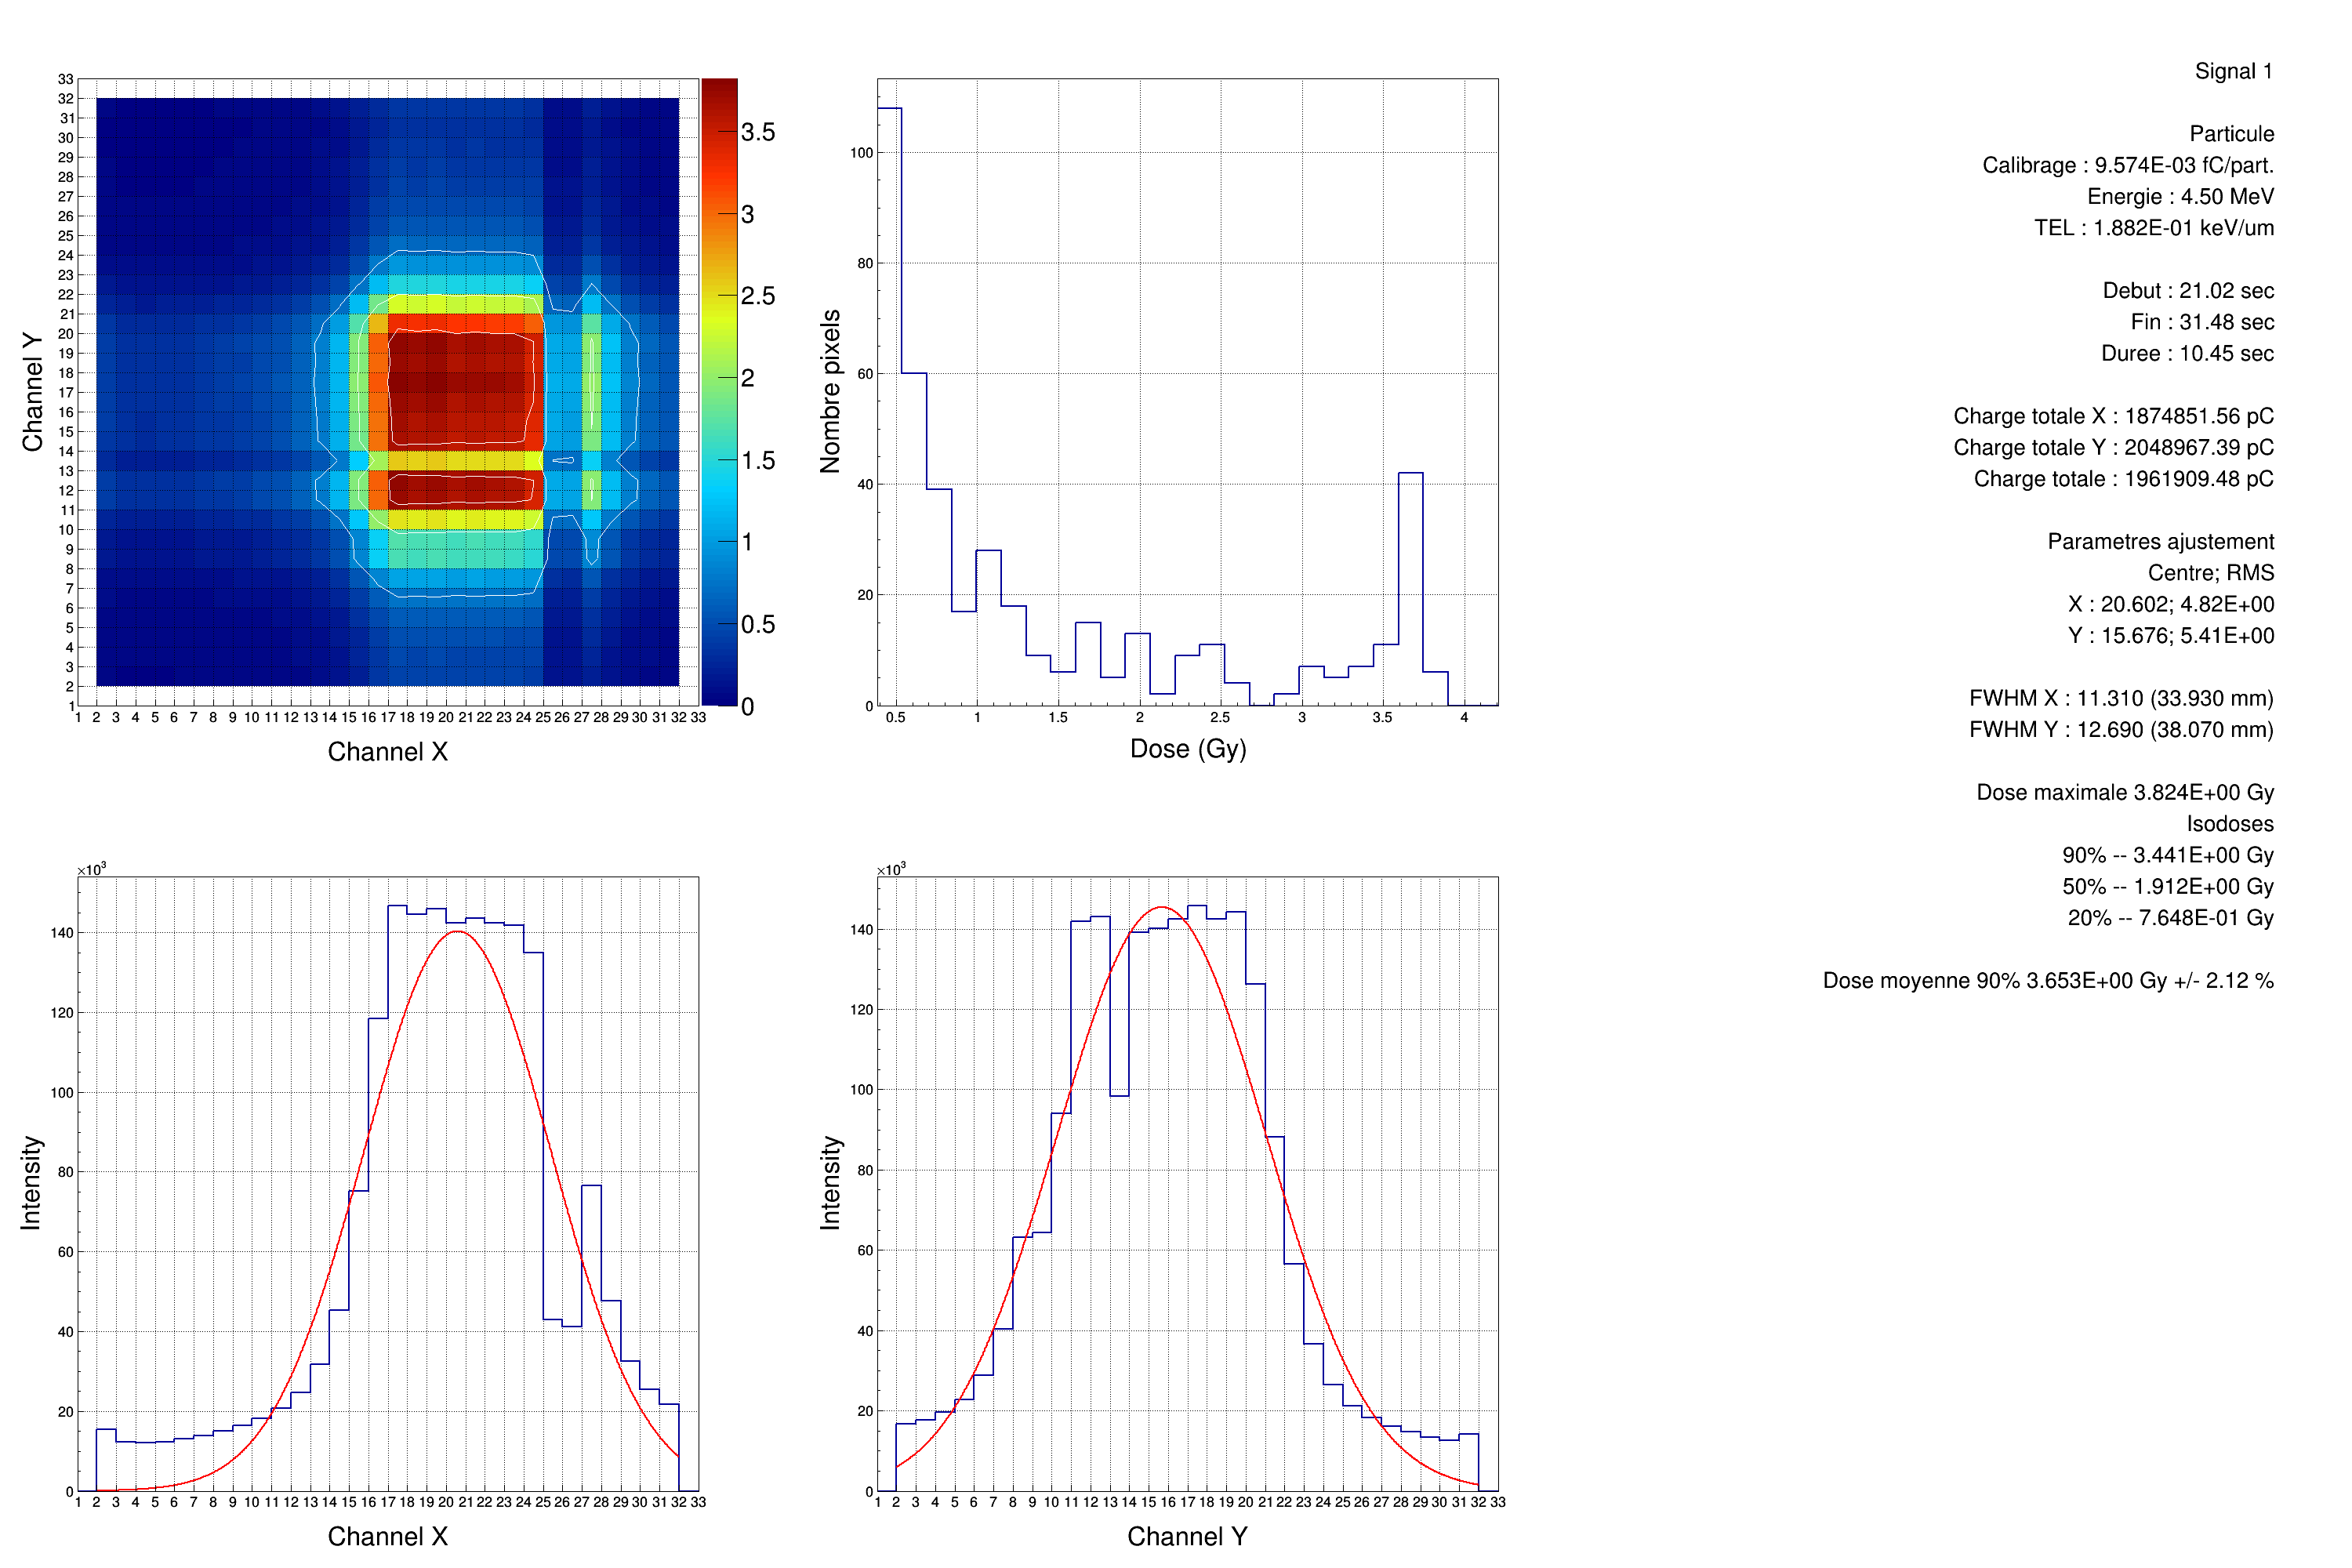
\includegraphics[width=\linewidth]{Area_1_sat.png} 
\caption{\label{fig:area_sat}\footnotesize{Résultats de l'analyse des données du Dosion de 3~mm obtenues lors de la 1$^{\text{ère}}$ irradiation}}
\end{center}
\end{figure}

Cette irradiation, ainsi que toutes les mesures issues du Dosion de 5~mm, est inexploitable et la seule "information" que nous pouvons en tirer est au final une description de $\ll$il se passe quoi quand ça sature$\gg$.

Lors de la deuxième irradiation, réalisée dans les mêmes conditions -- intensité, fréquence, position etc... -- un atténuateur, qui permet de diviser par 100 la charge reçue par les électromètres, a été placé sur le Dosion de 3~mm.
L'analyse nous donne des résultats qui semblent cohérents et sur lesquels nous ne distinguons pas de phénomène de saturation, figure \ref{fig:area_1_1000}.
\begin{figure}[h]
\begin{center}
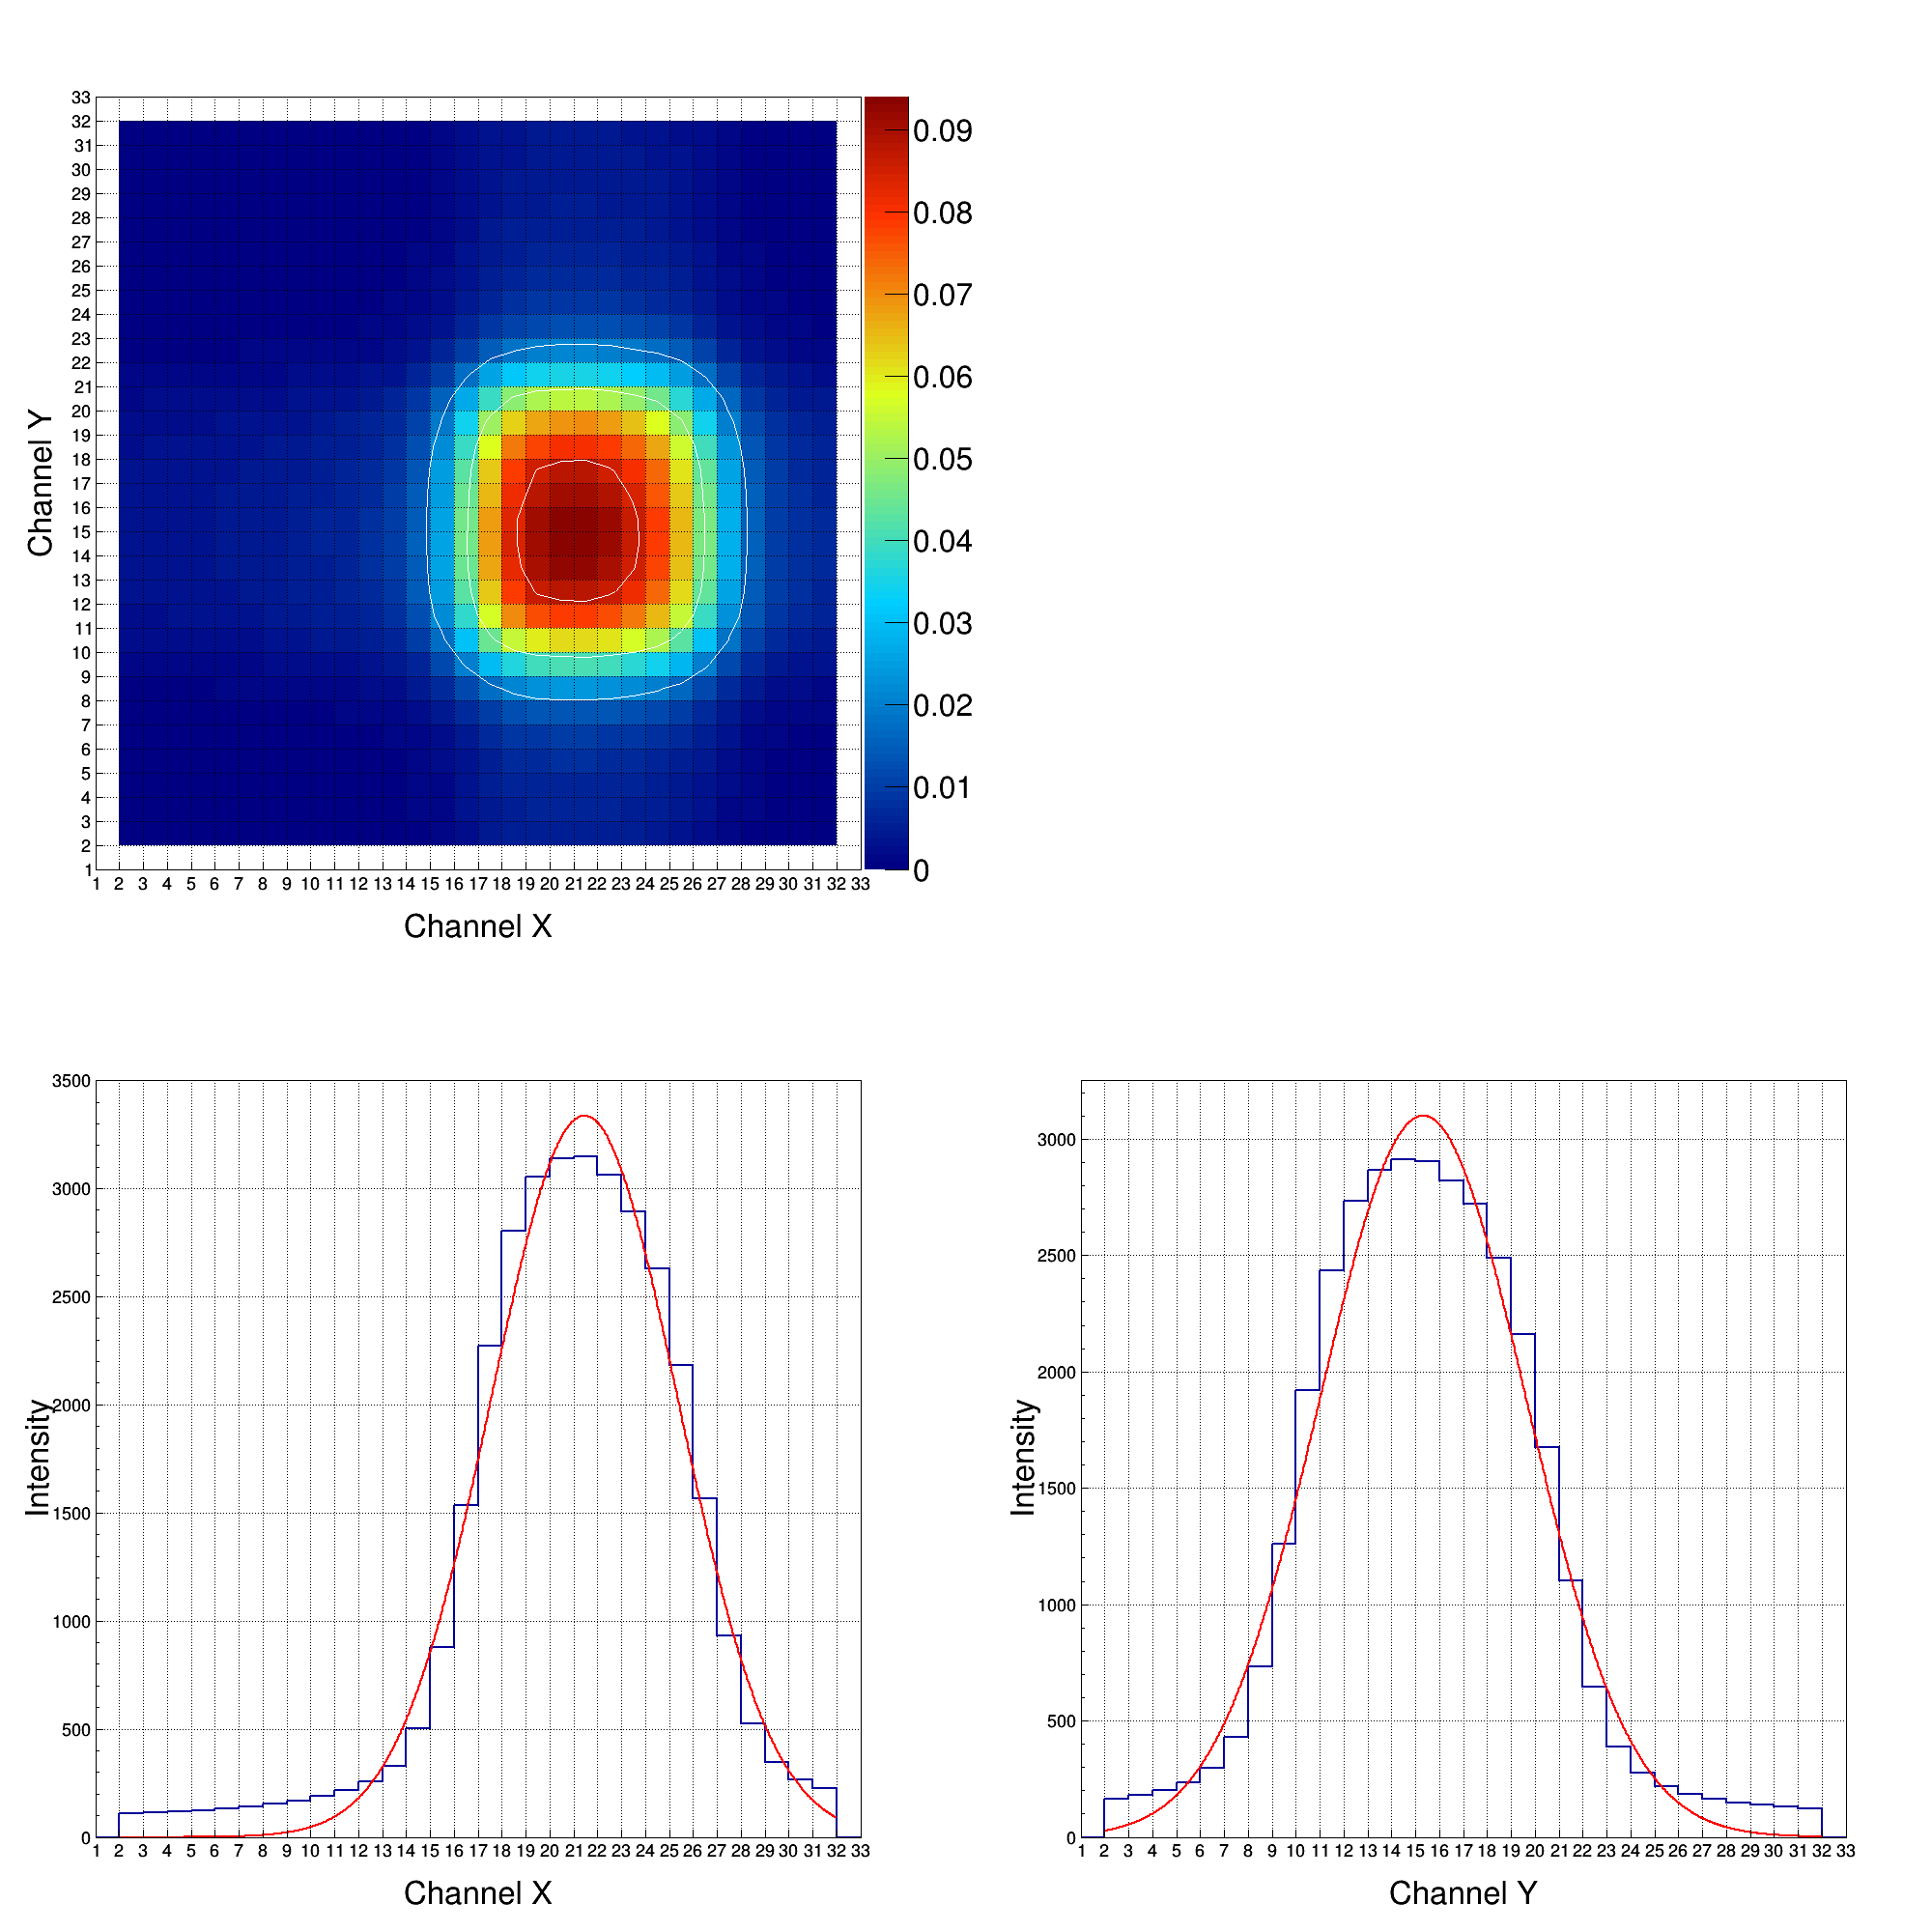
\includegraphics[width=\linewidth]{Area_1_1000.png} 
\caption{\label{fig:area_1_1000}\footnotesize{Résultats de l'analyse des données du Dosion de 3~mm équipé de l'atténuateur 100 et obtenues lors de la 2$^{\text{ème}}$ irradiation}}
\end{center}
\end{figure}

Nous remarquons notamment que le temps d'intégration des électromètres -- 2,4~ms (valeur qui peut descendre au plus bas à 40~$\mu$s) -- étant inférieur à la fréquence du pulse, nous pouvons observer chacun des 1000 pulses du Kinétron, figure \ref{fig:charge}.
Nous sommes donc capable d'analyser les données issues d'un seul pulse, figure \ref{fig:area_1_1}, et ainsi de constater qu'elles sont identiques, en considérant le facteur 1000, à celles obtenues sur toute la gamme temporelle, figure \ref{fig:area_1_1000}.
\begin{figure}[h]
\begin{center}
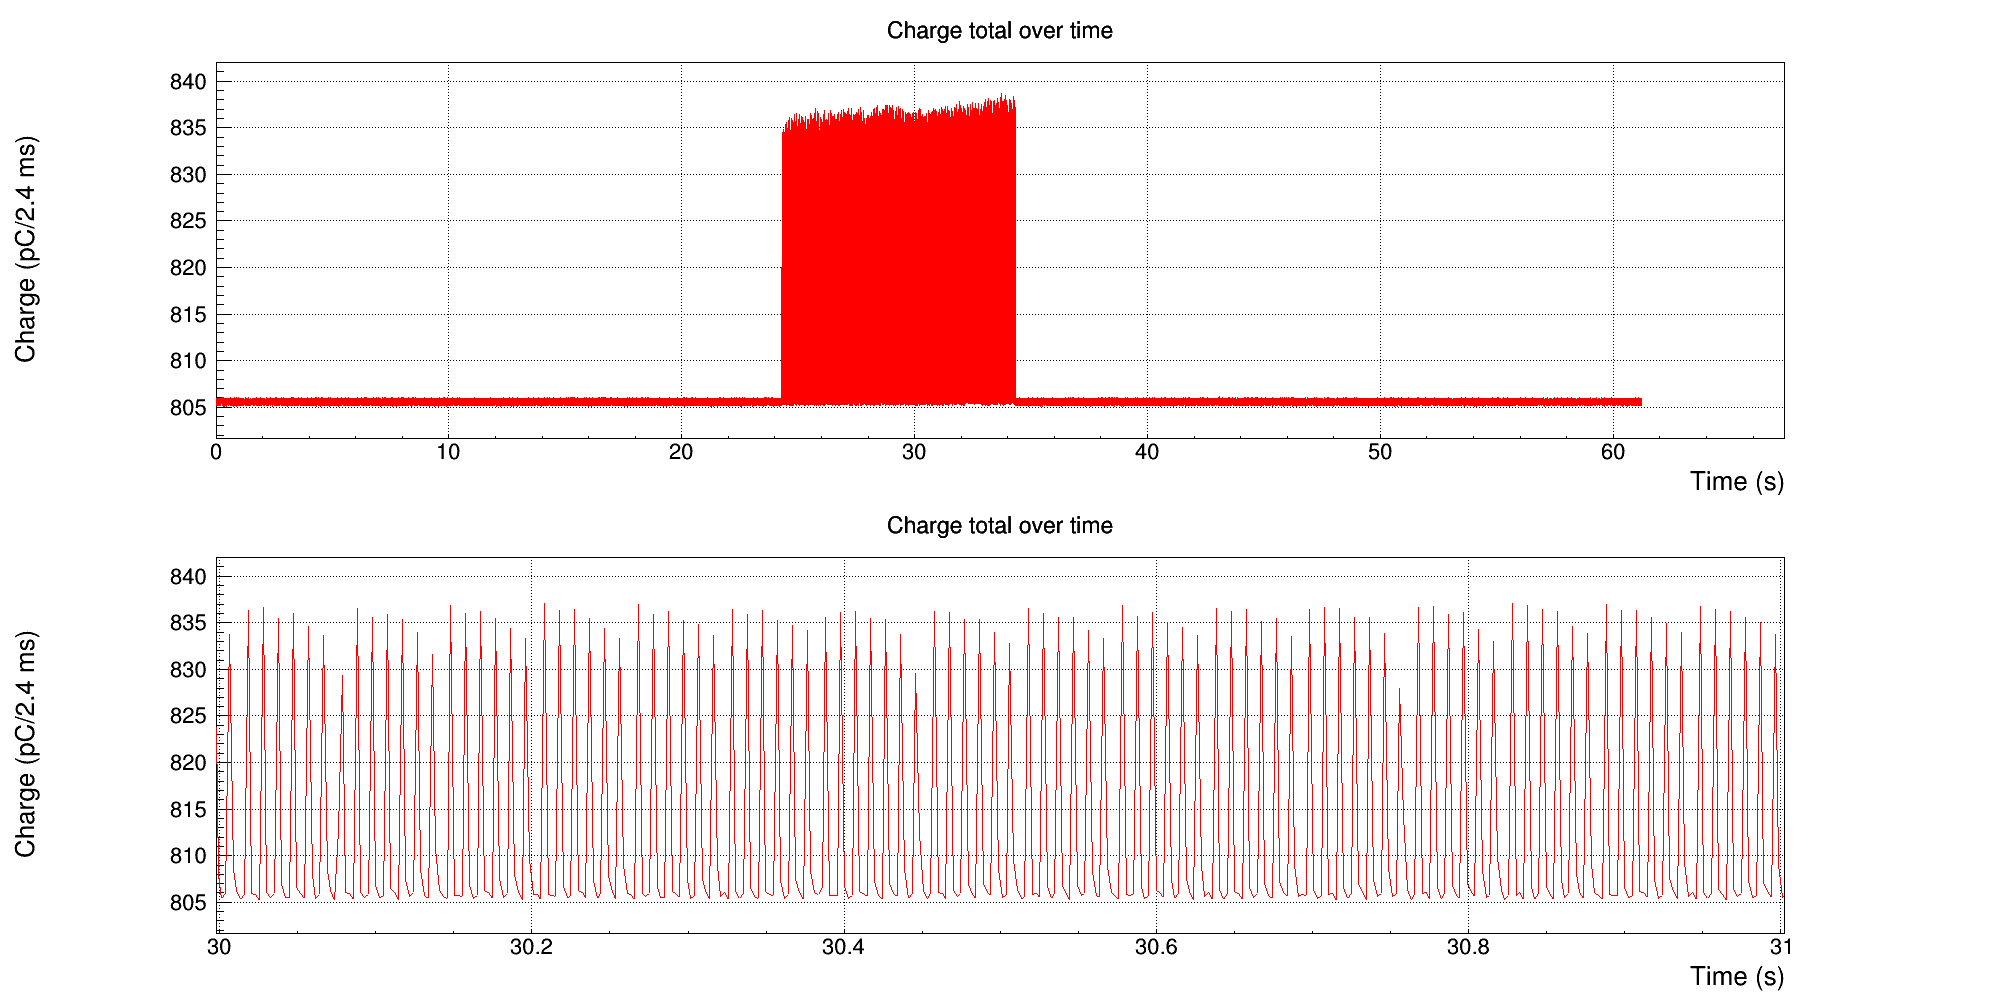
\includegraphics[width=\linewidth]{Charge.png} 
\caption{\label{fig:charge}\footnotesize{\'Evolution temporelle totale de l'irradiation et zoomée sur 1 seconde}}
\end{center}
\end{figure}

\begin{figure}[h]
\begin{center}
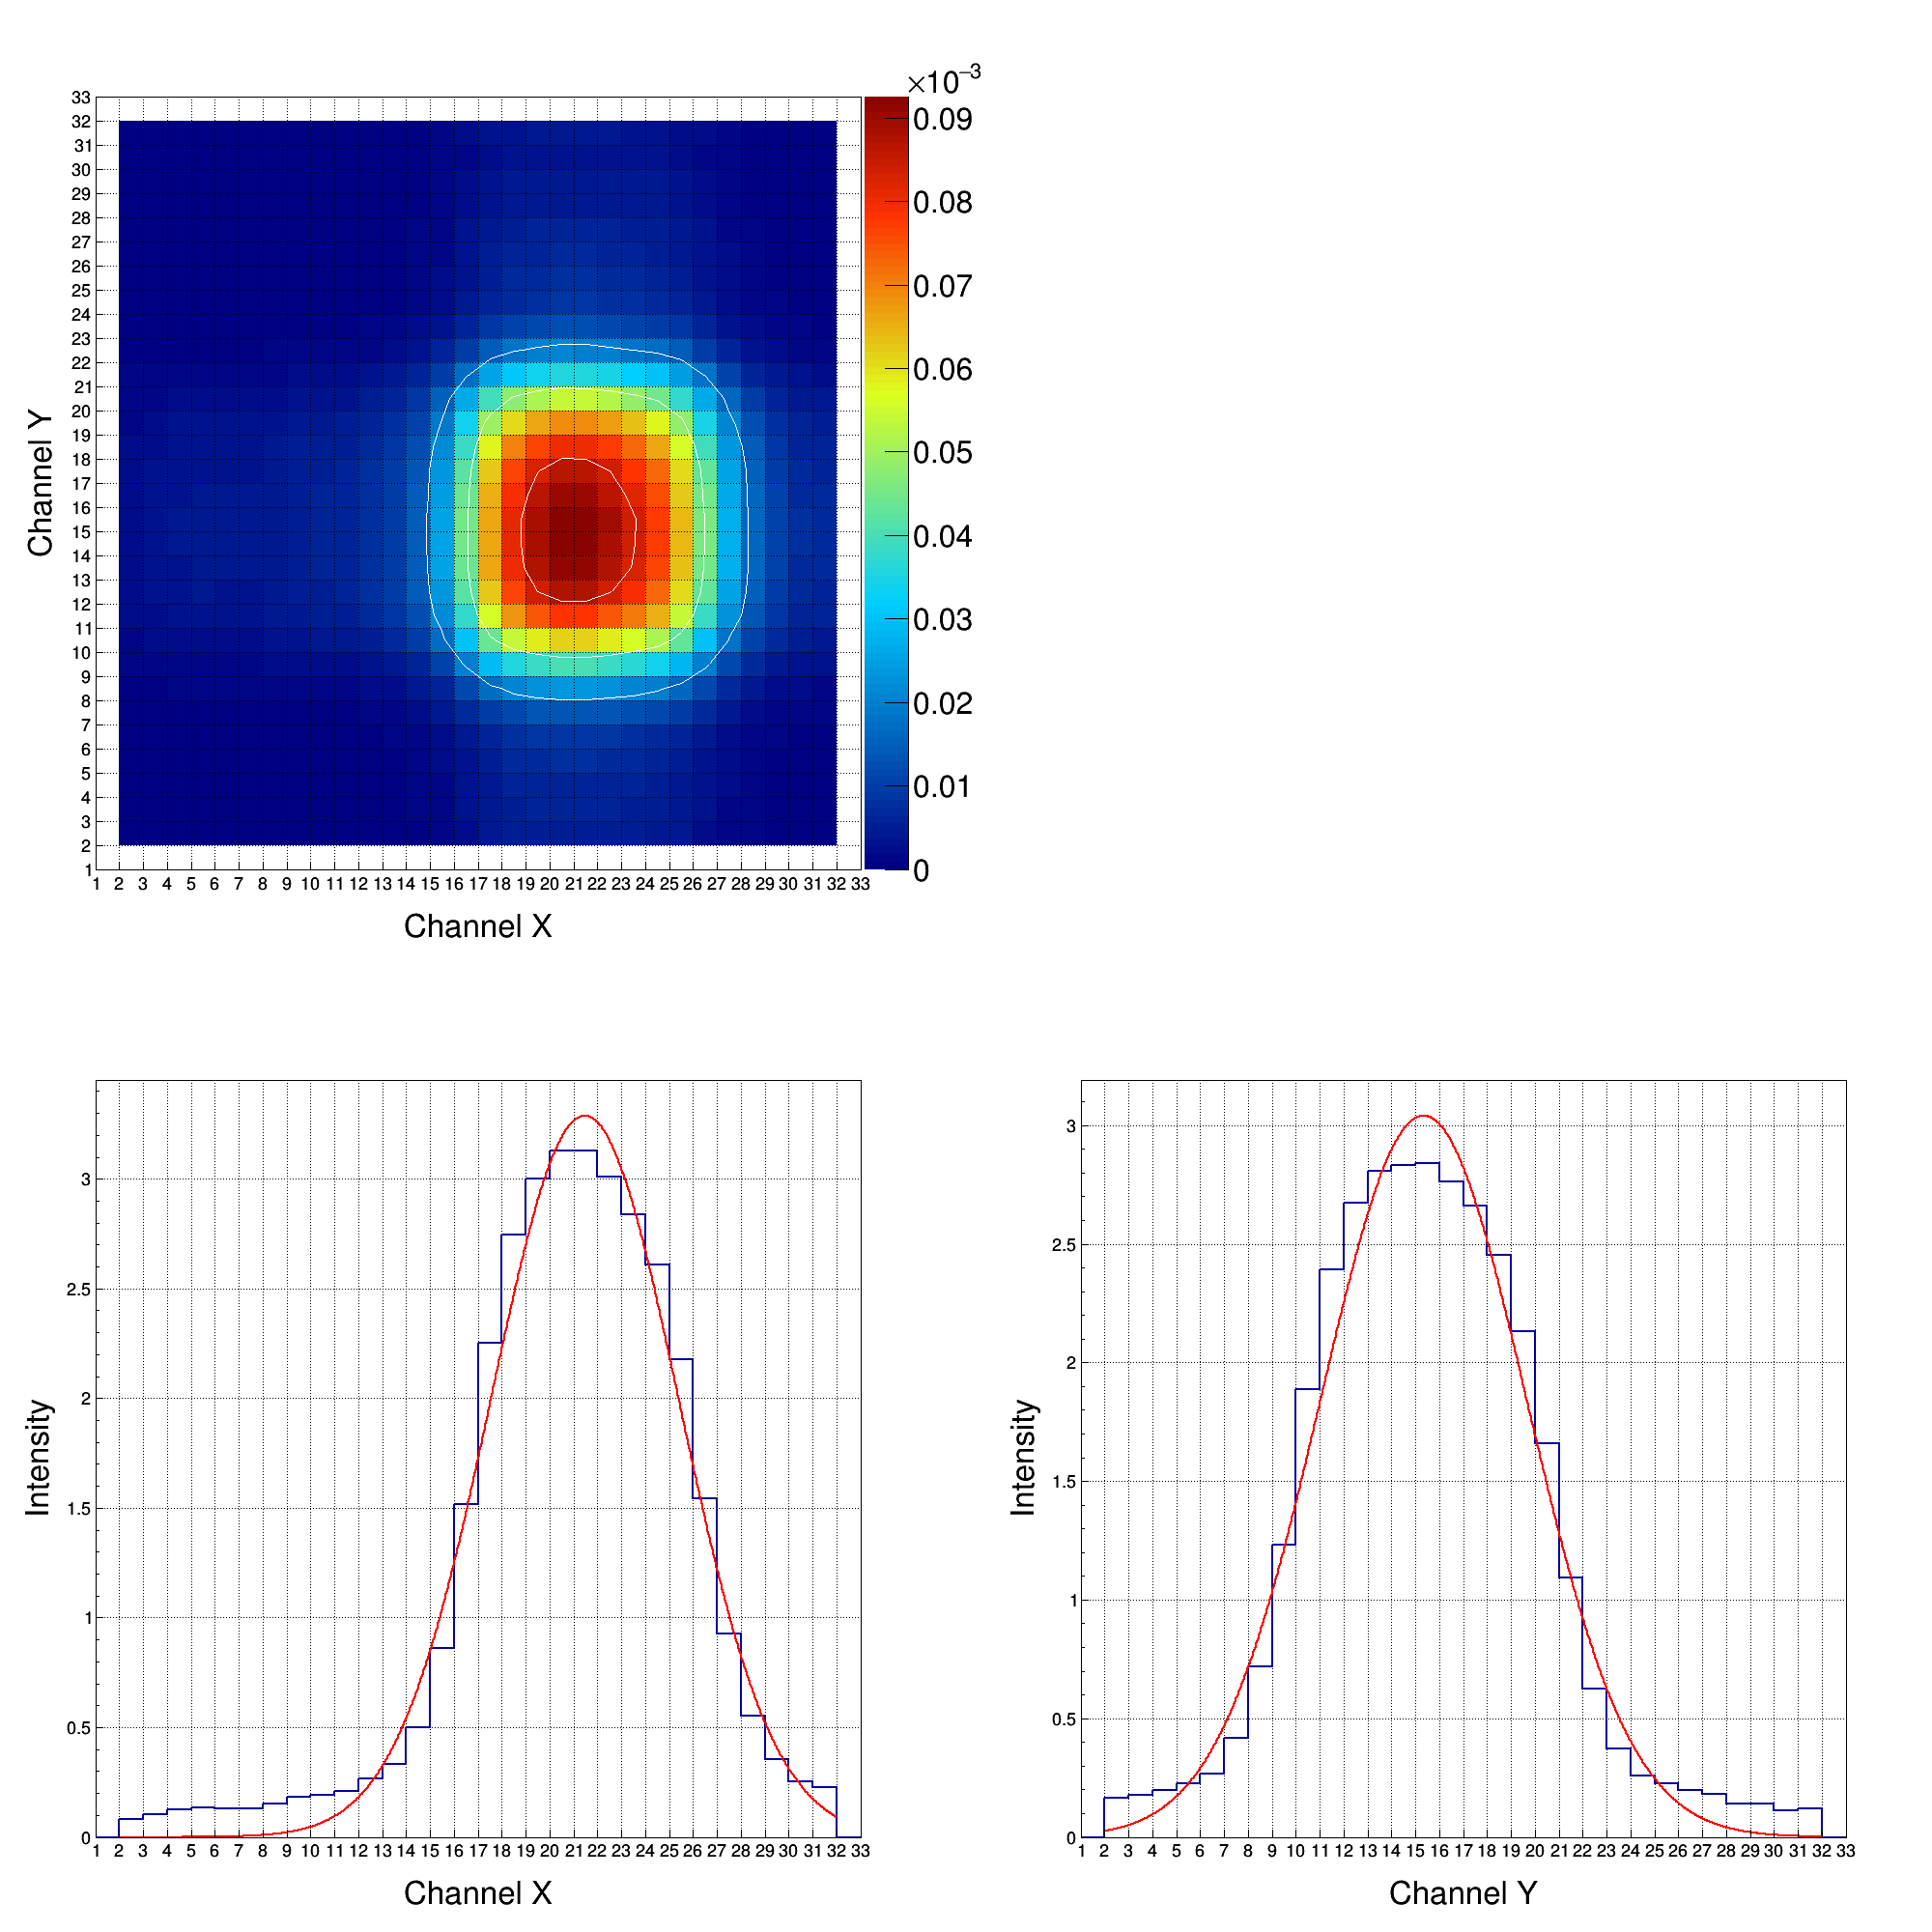
\includegraphics[width=\linewidth]{Area_1_1.png} 
\caption{\label{fig:area_1_1}\footnotesize{Résultats de l'analyse des données issues d'un seul pulse du Kinétron sur le Dosion de 3~mm équipé de l'atténuateur 100 et obtenues lors de la 2$^{\text{ème}}$ irradiation}}
\end{center}
\end{figure}


Les pistes externes du Dosion -- 1 à 15 puis 28 à 31 en X et 1 à 7 puis 21 à 31 en Y -- reçoivent moins de charges, étant hors de l'axe du faisceau, et sont donc moins sensibles au phénomène de saturation.
Nous pouvons alors les utiliser pour effectuer une normalisation des données afin de comparer les deux irradiations.
Lorsque nous superposons les valeurs obtenues durant ces deux premières irradiations sur le Dosion de 3~mm, en ayant pris soin d'appliquer le facteur de division de 100, nous remarquons bien le phénomène de saturation qui dégrade les valeurs obtenues lors de l'irradiation 1, figure \ref{fig:atté}.
\begin{figure}[h]
\begin{center}
\includegraphics[width=\linewidth]{Atténuation.png} 
\caption{\label{fig:atté}\footnotesize{Superposition des valeurs de charge obtenues, après normalisation sur les pistes externes, lors des deux premières irradiations avec et sans utilisation de l'atténuateur}}
\end{center}
\end{figure}

\newpage
De la même manière, la troisième irradiation, qui diffère par une intensité supérieure dans chaque pulse, a été comparée à la deuxième.
Nous pouvons remarquer, figure \ref{fig:ratio}, que si l'irradiation (2) est bien supérieure en intensité -- le rapport des charges indique un facteur de 16 en accord avec ce qui était attendu -- les normalisations, par rapport aux charges, ou au moyen des pistes externes, montrent une déformation de la gaussienne.
Cette déformation indique que là aussi nous avons atteint un niveau de saturation dans les électromètres.

\begin{figure}[h]
\begin{center}
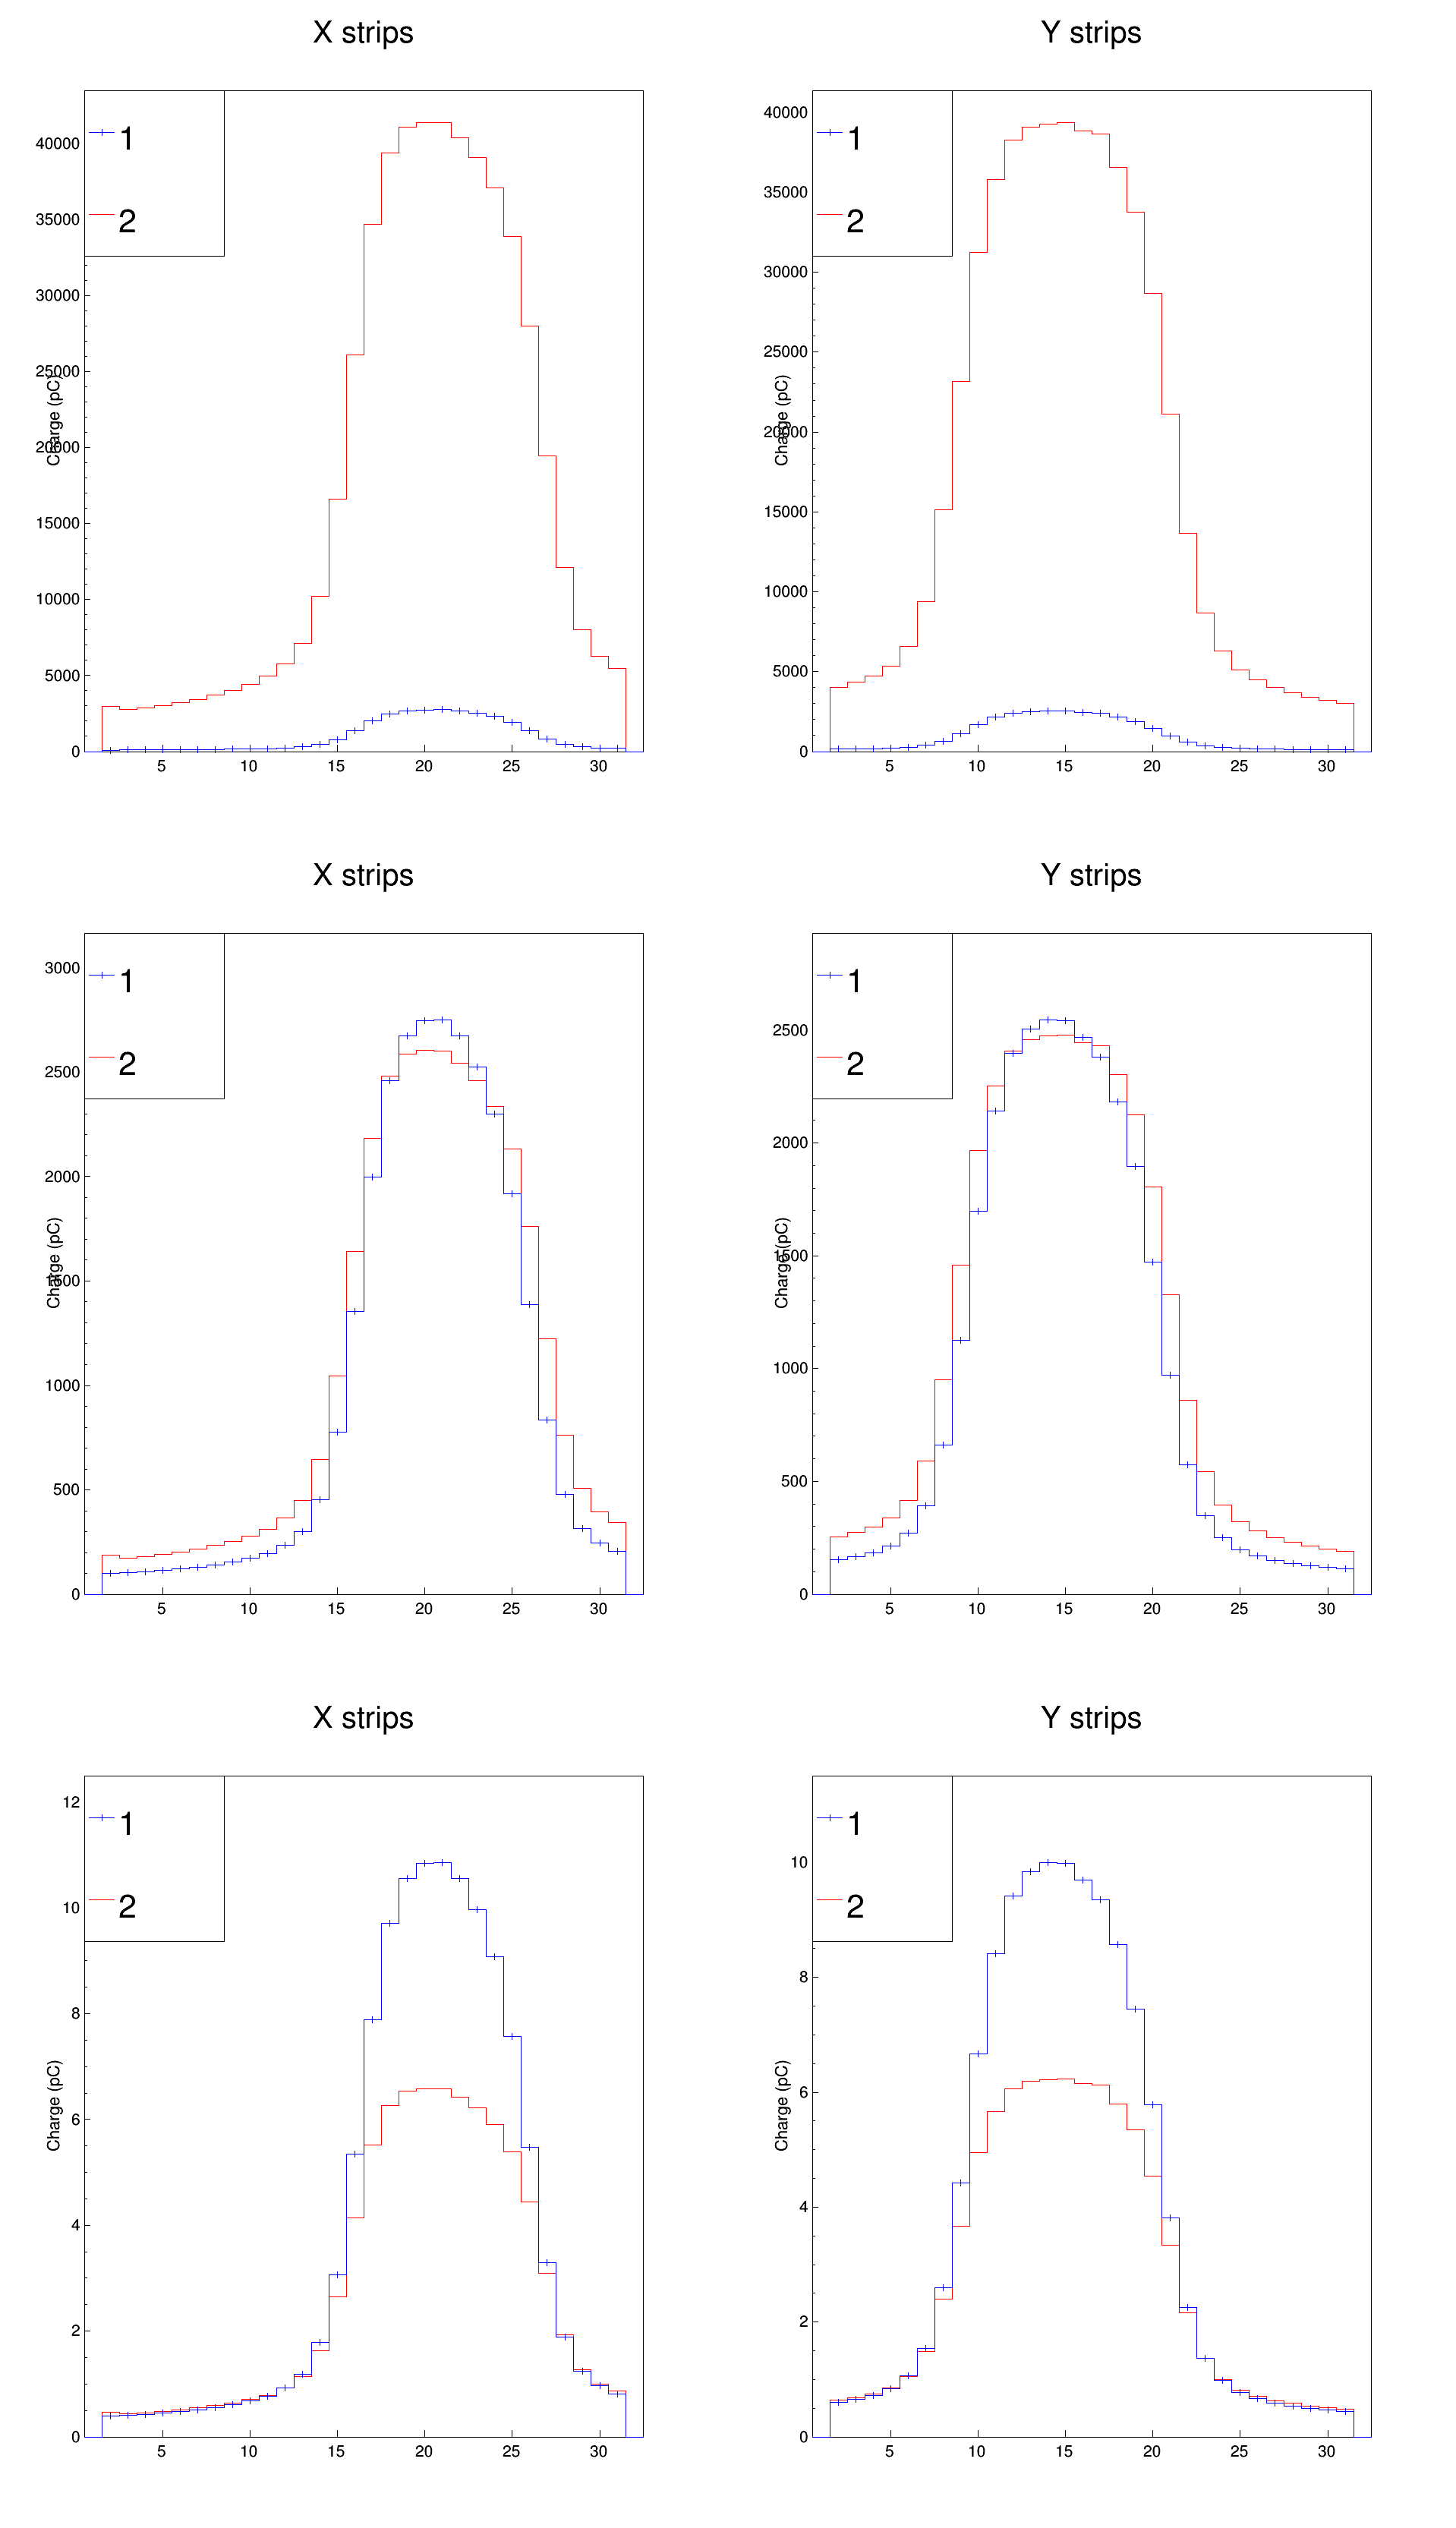
\includegraphics[width=0.8\linewidth]{Ratio_1_2_nn.png} 
\caption{\label{fig:ratio}\footnotesize{Superpositions des valeurs de charge obtenues lors des irradiations Dosion\_kinetron\_ate\_100\_1 (1) Dosion\_kinetron\_ate\_100\_2 (2) sans normalisation, en haut, avec une normalisation sur la charge totale, centre, et une normalisation sur les pistes externes, en bas}}
\end{center}
\end{figure}
Le facteur obtenu avec les pistes externes est lui de 25, donc un peu au delà des prévisions faites lors de l'irradiation. 
$\ll$il se passe quoi quand ça sature$\gg$
\newpage
\subsection*{Irradiations avec le PM}

Un scintillateur couplé à un photomultiplicateur a par la suite été utilisé.
Il doit nous donner une valeur de charges récoltées, qui dans son domaine de validité, est proportionnelle à l'intensité du faisceau.
Cela nous permettra ainsi, si la même proportionnalité est observée sur les charges de Dosion, de s'assurer que le phénomène de recombinaisons des charges n'est pas présent dans ce dernier.
Un total de 6 irradiations, pour 5 valeurs de tension de grilles différentes, a été réalisé.
Le bilan des valeurs de charges sur Dosion et le PM, ainsi que les ratios obtenus sont présentés dans la tableau \ref{tab:pmdosion}.
\`A noter que pour l'irradiation 6, la largeur du pulse était de 1~$\mu$s contre 100~ns pour les autres, et la tension du PM de 800~V contre 1000~V ce qui a diminué la charge collectée.

\begin{table}
\begin{center}
\begin{tabular}{l|rrrrrr}
Irradiation&1&2&3&4&5&6\\
Tension grille (V)&50&80&90&100&150&150\\
\hline
Charge PM (u.a)&4692&4852	&5788&6339&6381&5854\\
Charge Dosion (u.a)&37558&37995&48061&67316&317863&1353739\\
Ratio PM/Dosion&0.1249&0.1277&0.1204&0.0942&0.0201&0.0043\\
\hline
\end{tabular}
\caption{\label{tab:pmdosion}\footnotesize{Récapitulatif des charges mesurées, en unité arbitraire, pour le PM et Dosion sur les 6 irradiations, ainsi que le ratio calculé}}
\end{center}
\end{table}

Nous notons que pour les 3 premières irradiations nous obtenons un ratio constant.
Par la suite, et comme observé lors des tirs, le PM sature ce qui le rend lui aussi inexploitable.

Nous pouvons effectuer le même type de comparaison que précédemment pour les valeurs issues de Dosion, figure \ref{fig:ratio_PM}.
Nous y observons qu'à partir de la 4$^{\text{ème}}$ irradiation un phénomène de saturation apparaît.
Ce qui semble intéressant c'est que celui-ci est visible uniquement suivant les pistes X.
Cela s'explique car le faisceau étant moins diffusé suivant l'axe X, figure \ref{fig:area_1_1000}, le nombre de pistes et donc d'électromètres sollicités est moindre donc la saturation y apparaît plus "tôt" que pour les pistes Y.
\begin{figure}[h]
\begin{center}
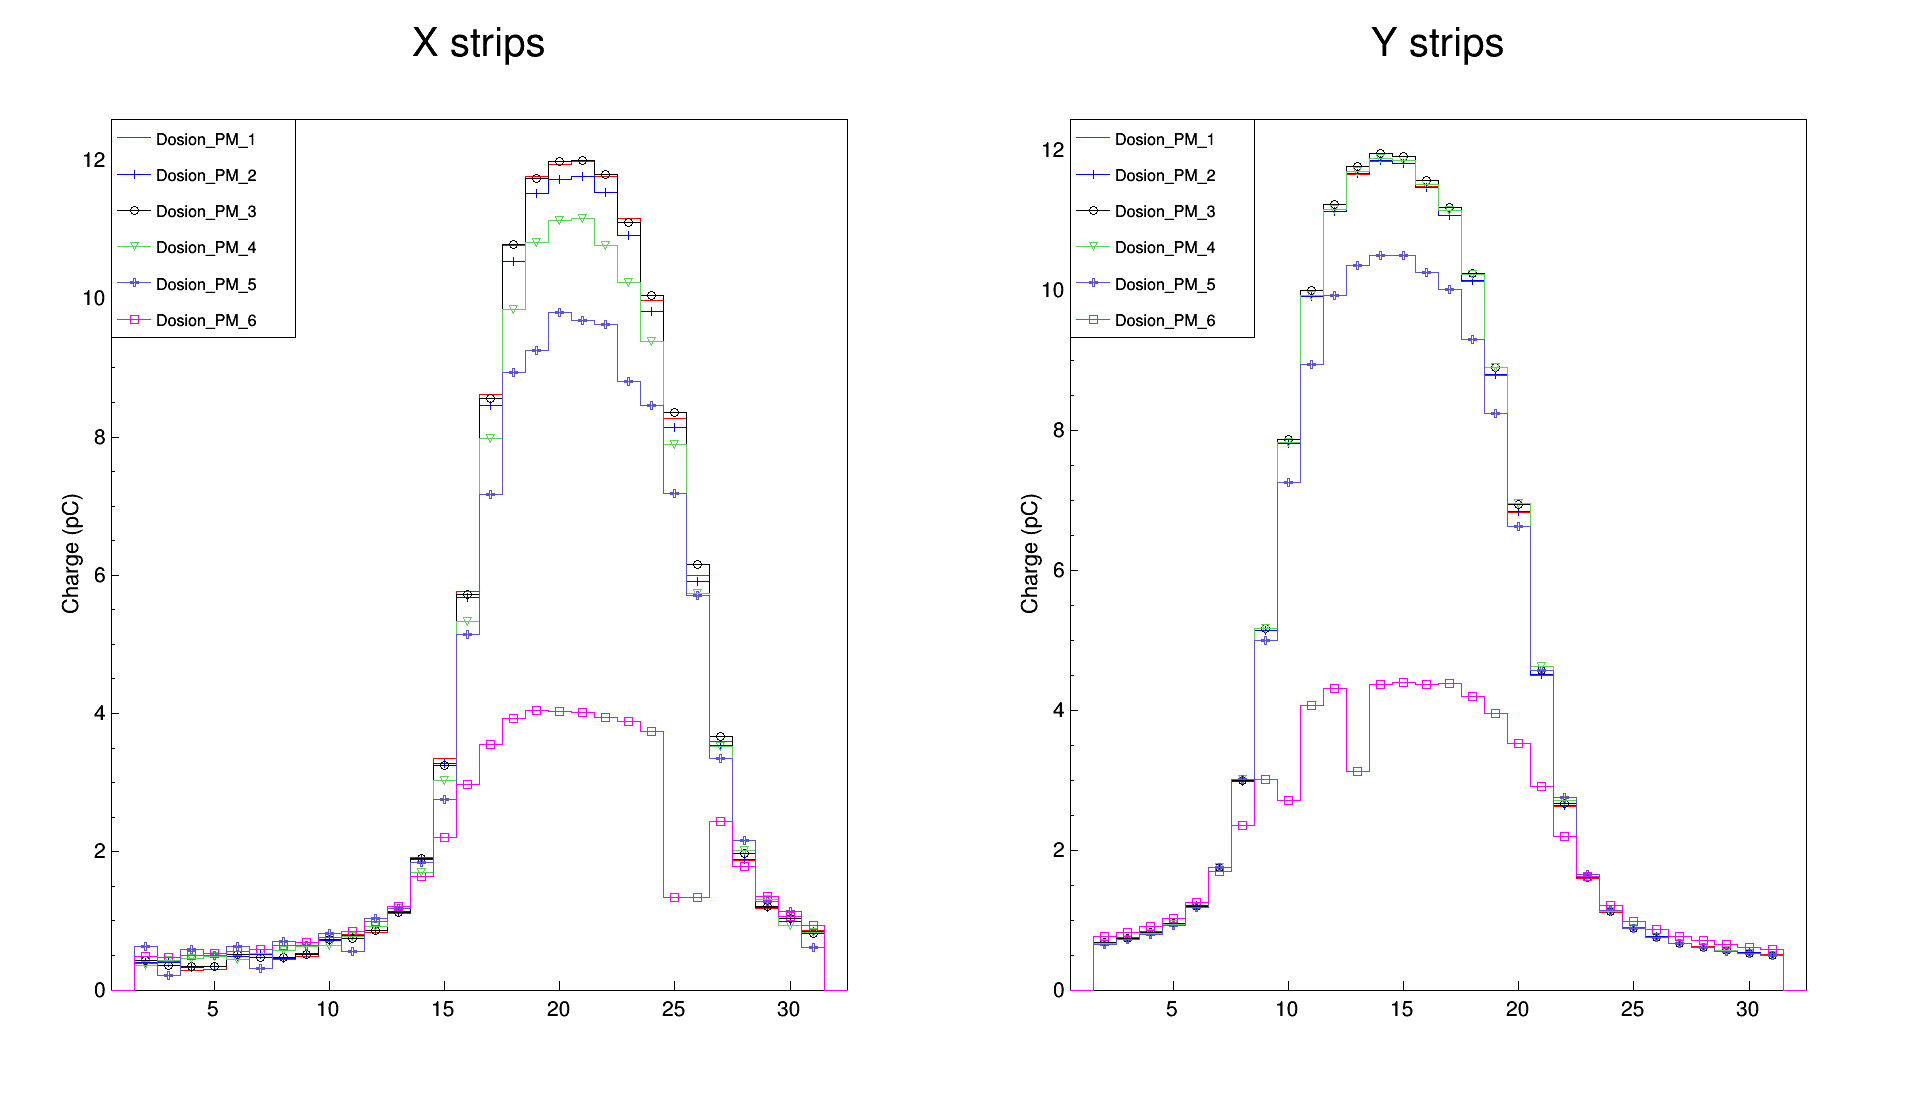
\includegraphics[width=\linewidth]{Dosion_PM.png} 
\caption{\label{fig:ratio_PM}\footnotesize{Superpositions des valeurs de charge obtenues lors des 6 irradiations Dosion\_PM et normalisées suivant les pistes externes}}
\end{center}
\end{figure}

L'analyse de la dernière irradiation, figure \ref{fig:area_pm}, nous montre des résultats très semblables à ceux obtenus pour la première, figure \ref{fig:area_sat}.
Cela semble indiquer, suivant la fameuse observation du $\ll$il se passe quoi quand ça sature$\gg$, que là encore c'est principalement un soucis de saturation des électromètres qui dégrade la mesure et non une recombinaison des charges dans la chambre.
\begin{figure}[h]
\begin{center}
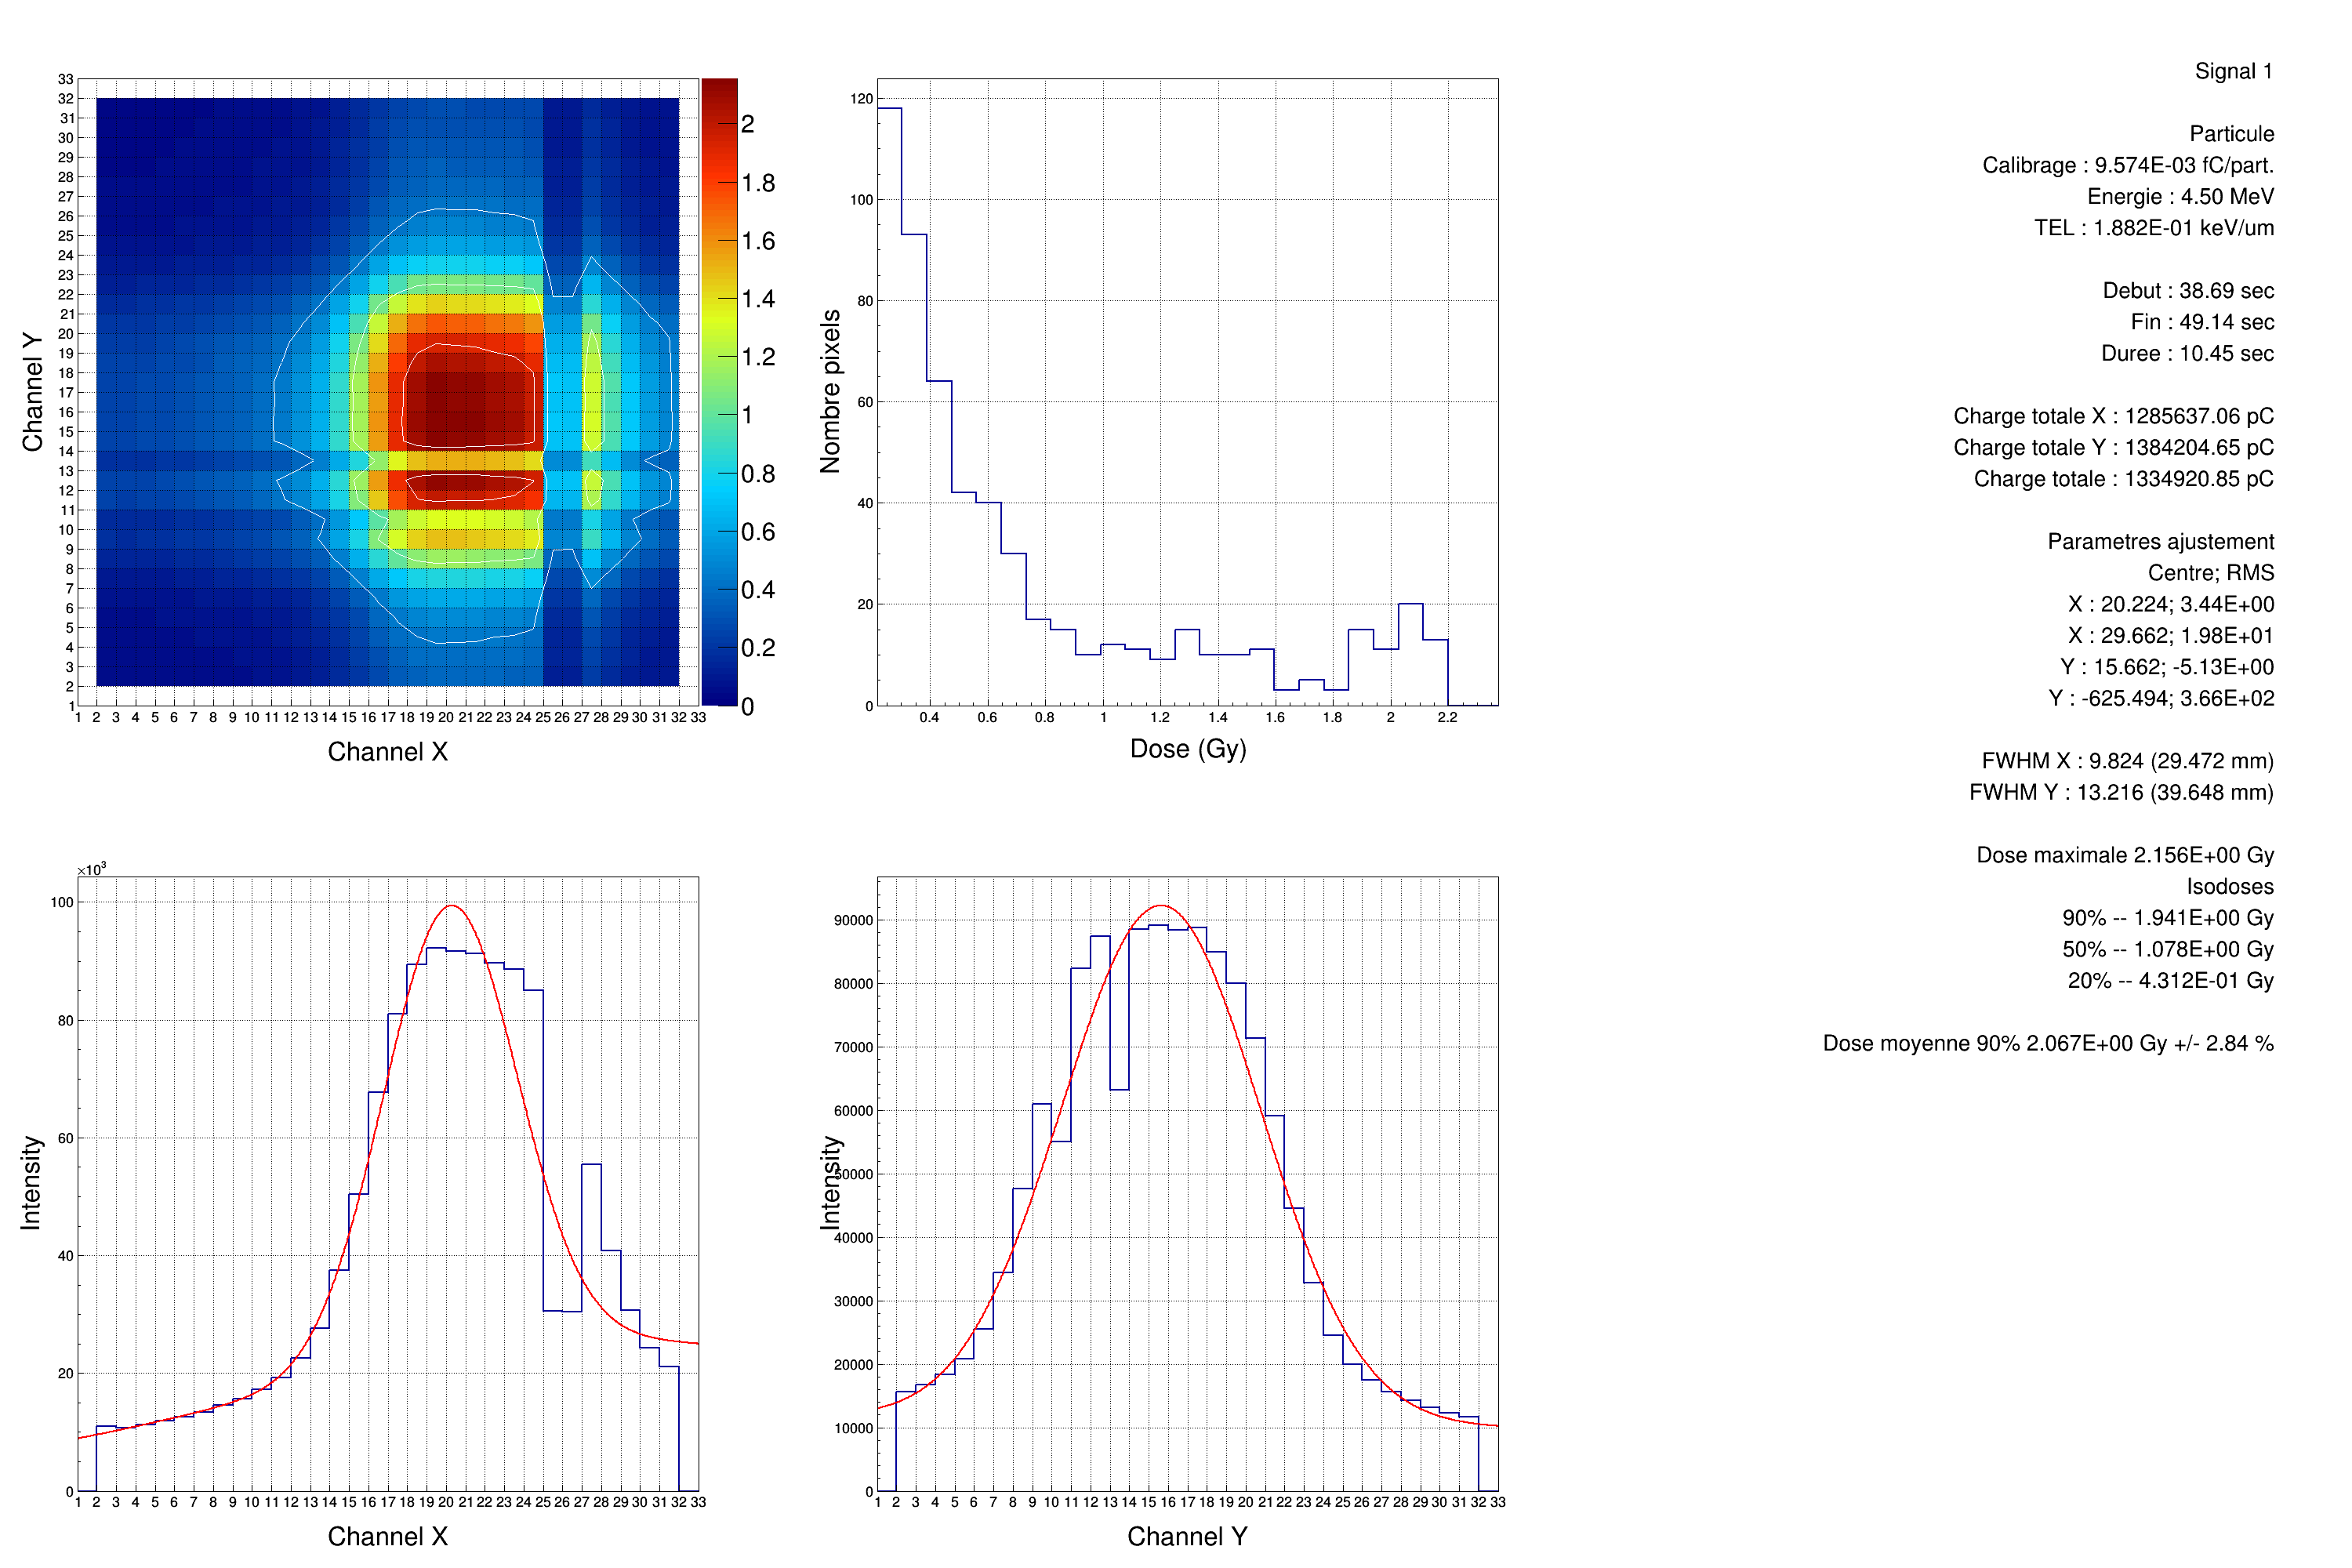
\includegraphics[width=\linewidth]{Area_1_PM_6.png} 
\caption{\label{fig:area_pm}\footnotesize{Résultats de l'analyse des données du Dosion de 3~mm obtenues lors de la dernière irradiation avec une tension de grille de 150 V, une largeur de pulse de 1~$\mu$s pour une fréquence de 100~Hz}}
\end{center}
\end{figure}
\`A noter qu'en utilisant les valeurs de dose obtenues pour les premières irradiations et le facteur de normalisation calculé pour la courbe \ref{fig:area_pm}, la dose totale délivrée lors de cette dernière irradiation a été estimée à environ 80~Gy/s.
Ajoutons que le facteur de normalisation confirme bien que l'intensité y était 10 fois supérieure à l'irradiation 5.

\clearpage
\subsection*{Perspectives}

Cette première journée d'irradiations nous a surtout permis de découvrir l'installation du Kinétron et d'y tester Dosion.
De nombreux points méritent d'être explorés plus en détails.

Tout d'abord obtenir une mesure de la dose par l'intermédiaire d'un autre détecteur nous conforterait dans la robustesse de notre méthode et nous fournirait un point de comparaison.
Nous pouvons utiliser la chambre PTW que nous n'avions pas eu le temps de mettre en place la dernière fois.

L'utilisation de l'atténuateur 10000 va nous permettre d'élargir la gamme de fonctionnement et d'ainsi se rapprocher des intensités où le phénomène de recombinaison pourrait se produire.
Le PM nous permettra encore de tester la validité de Dosion, de la même façon que détaillée plus haut.
Cependant nous utiliserons le plastique de 2~mm (contre 5~mm) et nous le placerons à un endroit moins sensible aux diffusions.
Faire évoluer la tension du PM sera également indispensable pour garder son comportement exploitable aux plus hautes intensités.

Je ne sais pas quelles sont les limites du Kinétron en terme de tension de grille, largeur de pulse et fréquence ?

Faire évoluer la largeur du pulse présenterait un intérêt moindre étant donné qu'elle sera toujours bien inférieure à la limite temporelle de 40~$\mu$s -- deux fois 20~$\mu$s -- des électromètres (sauf si cela permet d'augmenter la quantité d'électrons par pulse dans le cas où la tension de grille serait à son maximum).
En revanche jouer sur la tension de grille, comme précédemment, en maîtrisant mieux la réponse du PM, et augmenter la fréquence permettraient d'éprouver les limites de Dosion.

La mobilité des ions est d'environ 200~mm$^2\cdot$V$^{-1}\cdot$s$^{-1}$ dans l'air.
Pour un champ électrique de 900~V sur 3~mm, cela donne une vitesse de déplacement de 60~$\mu$m$\cdot\mu$s$^{-1}$.
Ils ont ainsi besoin de 50~$\mu$s -- 30~$\mu$s si nous augmentons la tension dans Dosion à 1500~V -- pour être totalement collectés.
Cela suppose que jusqu'à une fréquence de pulse à 20~kHz nous devrions éviter un "empilement" des charges dans la chambre, phénomène qui augmente leurs probabilités de recombinaisons (voire conduit à un effondrement du champ).

Ce sont bien sûr des points qu'il faut valider expérimentalement.

Pour résumer, les points à étudier pour une prochaine fois sont :
\begin{itemize}
\item l'obtention d'une mesure de dose par un autre détecteur (PTW ou autre) ;
\item l'utilisation de manière plus efficace du PM ;
\item faire varier la tension de grille (ou la largueur du pulse) et/ou
\item la fréquence du pulse jusqu'à une possible recombinaison des charges dans la chambre ;
\item augmenter ces paramètres jusqu'à atteindre la saturation des électromètres (avec atténuateur 10000).
\end{itemize}

%%%%%%%%%%%%%%%%%%%%%%%%%%%%%%%%%%

\end{document}

%%%%%%%%%%%%%%%%%%%%%%%%%%%%%%%%%%%%%%%%%%%%%%%%%%%%%%%%%%%%%%%%%%%%%%%%%%%%%%%%%%%%%%%%%%%%%%%%%%